Der Client stellt die Anwendung dar, mit der ein Nutzer aktiv als Spieler oder auch passiv als Gast an einer Partie teilnehmen kann.

\subsubsection{Schnittstellenarten}
Als Benutzerschnittstelle wird eine grafische Benutzeroberfläche verwendet. \\ \textbf{Begründung:} Um das Spiele so intuitiv wie möglich zu gestalten, ist es sinnvoll, dem Nutzer alle für das Spielgeschehen relevanten Informationen und Aktionen grafisch in einer GUI darzustellen. Hinzu kommt, dass neben dem eigentlichen Spiel auch die zugehörigen Funktionen, wie zum Beispiel das Verbinden mit einem Server, benutzerfreundlich und leicht zu bedienen sein sollte. Dies lässt sich am leichtesten durch eine grafische Benutzeroberfläche bewerkstelligen.

\newpage

\subsubsection{Dialoge}
Im Folgenden sind alle Dialoge, die während der Nutzung des Clients benötigt werden, den zugehörigen Anwendungsfällen zugeordnet. 

\begin{figure}[H]
    \centering
    \begin{tabular}{|p{\textwidth/4} p{\textwidth/12} p{\textwidth/16} p{\textwidth/2}|}
        \hline
        \textbf{Name} & \textbf{Typ} & \multicolumn{2}{l|}{\textbf{Abgedeckte Anforderungen}} \\\hline
        Startbildschirm & Dialog & FA60 & Hauptmenü [Ansicht]\\\hline
        Hilfe & Dialog & FA65 & Hilfe [Ansicht]\\
        & & QA18 & Benutzerfreundlichkeit\\\hline
        Hotkey-Liste & Dialog & FA65 & Hilfe [Ansicht]\\
        & & FA68 & Hotkeys\\\hline
        Team ändern & Popup & FA63 & Team-Konfiguration importieren [Ansicht]\\
        & & FA15 & Teams\\
        & & FA54 & Quidditchtem-Konfiguration\\
        & & FA61 & Spiel beitreten [Ansicht]\\\hline
        Beenden & Popup & & \\\hline
        Spielstart fehlgeschlagen & Popup & QA16 & Zuverlässigkeit\\\hline
        Verlassen & Popup & &\\\hline
        Spielsuche & Dialog & FA61 & Spiel beitreten [Ansicht]\\
        & & FA55 & Netzwerkschnittstelle\\\hline
        Spielende & Dialog & FA62 & Spiel Ende [Ansicht]\\
        & & FA49 & Spielende\\\hline
        Beobachten & Dialog & FA66 & Beobachter [Ansicht]\\\hline
        Verbindungsabbruch & Dialog & QA16 & Zuverlässigkeit\\
        & & QA17 & Robustheit\\\hline
        Pause & Dialog & FA69 & Pausieren\\\hline
    \end{tabular}
\end{figure}
\begin{figure}[H]
    \centering
    \begin{tabular}{|p{\textwidth/4} p{\textwidth/12} p{\textwidth/16} p{\textwidth/2}|}
        \hline
        Spiel & Dialog & FA64 & Spiel[Ansicht]\\
        & & FA1 & Spielfeld\\
        & & FA2 & Mittelkreis\\
        & & FA3 & Mittelzelle\\
        & & FA4 & Hüterzone\\
        & & FA5 & Zelle\\
        & & FA6 & Torring\\
        & & FA8 & Punkte erzielen\\
        & & FA10 & Ball\\
        & & FA11 & Quaffel [Ball]\\
        & & FA12 & Klatscher [Ball]\\
        & & FA13 & Goldener Schnatz [Ball]\\
        & & FA14 & Besen\\
        & & FA16 & Spielfiguren\\
        & & FA17 & Jäger\\
        & & FA18 & Treiber\\
        & & FA19 & Hüter\\
        & & FA20 & Sucher\\
        & & FA31 & Fans\\
        & & FA32 & Elfen [Fantyp]\\
        & & FA33 & Kobolde [Fantyp]\\
        & & FA34 & Trolle [Fantyp]\\
        & & FA35 & Niffler [Fantyp]\\
        & & FA36 & Schiedsrichter\\
        & & FA44 & Runde\\
        & & FA46 & Spielerphase\\\hline
    \end{tabular}
\end{figure}

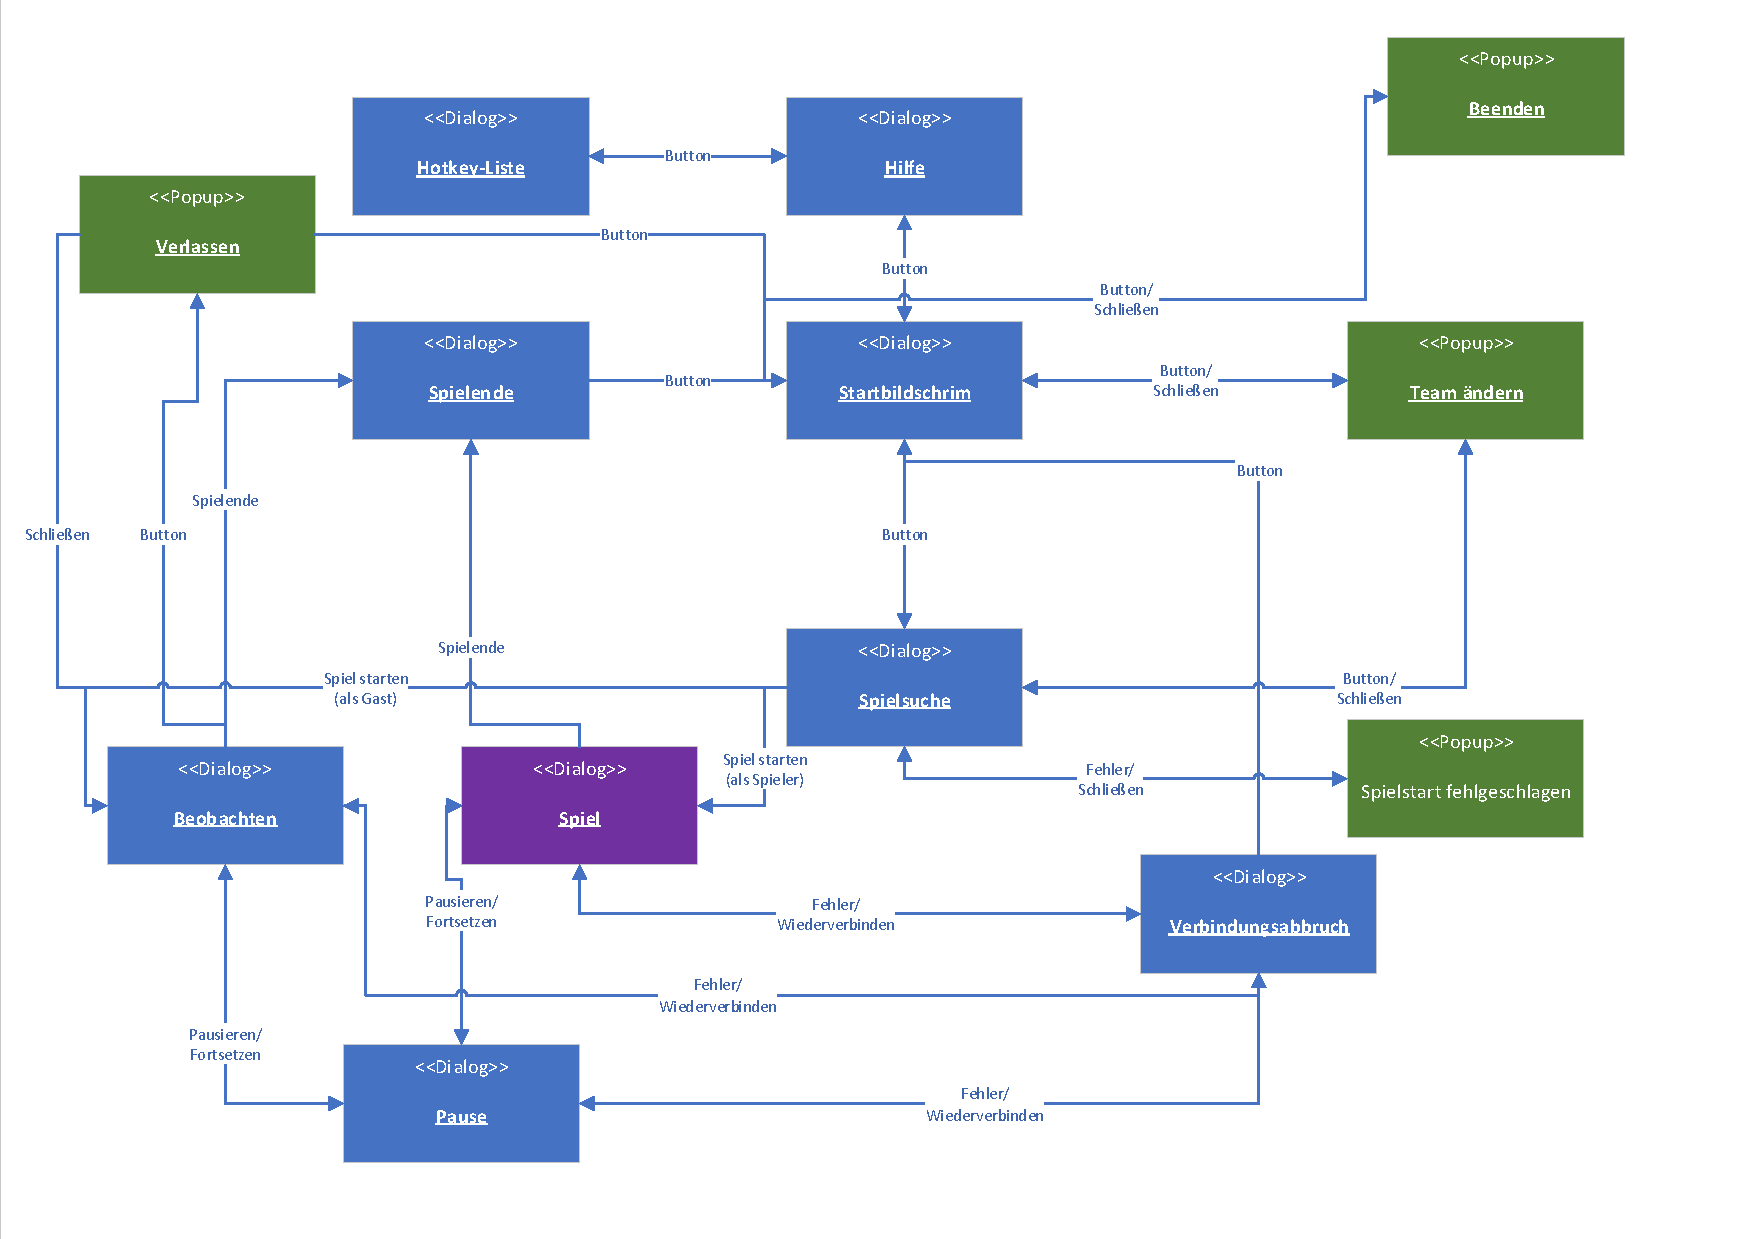
\includepdf[pages=-, scale=0.8, pagecommand={\subsubsection{Dialogstrukturdiagramme}}]{../Meilenstein03/images/Client_Hauptmenue.pdf}
